\documentclass[twocolumn, 11pt]{article}%
\usepackage{amsmath, amssymb, esint, gensymb, hyperref}
\usepackage{graphicx, cuted, geometry, float, chemfig}

\geometry{
    a4paper,
    total={170mm,260mm},
}

\begin{document}

\begin{strip}
  \vspace*{\dimexpr-\stripsep}
  \begin{center}
      \Large\textbf{FISIKA 2}\\
      \large{Pertemuan 1 - Minggu 2 (722465)}\\
      \large{\today}
   \end{center}
\end{strip}

\section{ASISTENSI}
    Soal diurutkan berdasarkan urutan materi..\\
    Selamat berlatih, Happy Tinkering Nerds!!

    \begin{center}
        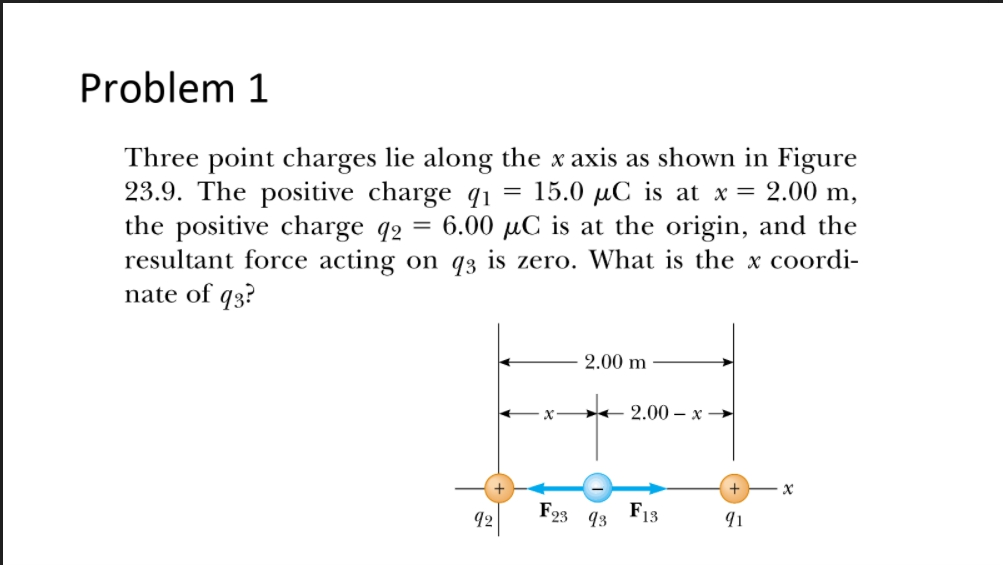
\includegraphics[width=225px]{1.jpg}
    \end{center}

    \begin{center}
        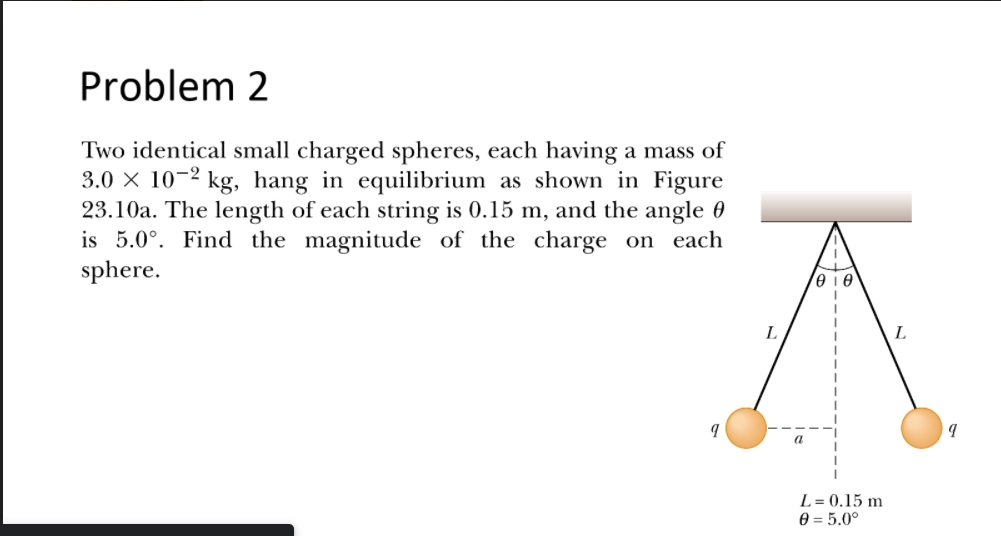
\includegraphics[width=225px]{2.jpg}
    \end{center}

    \begin{center}
        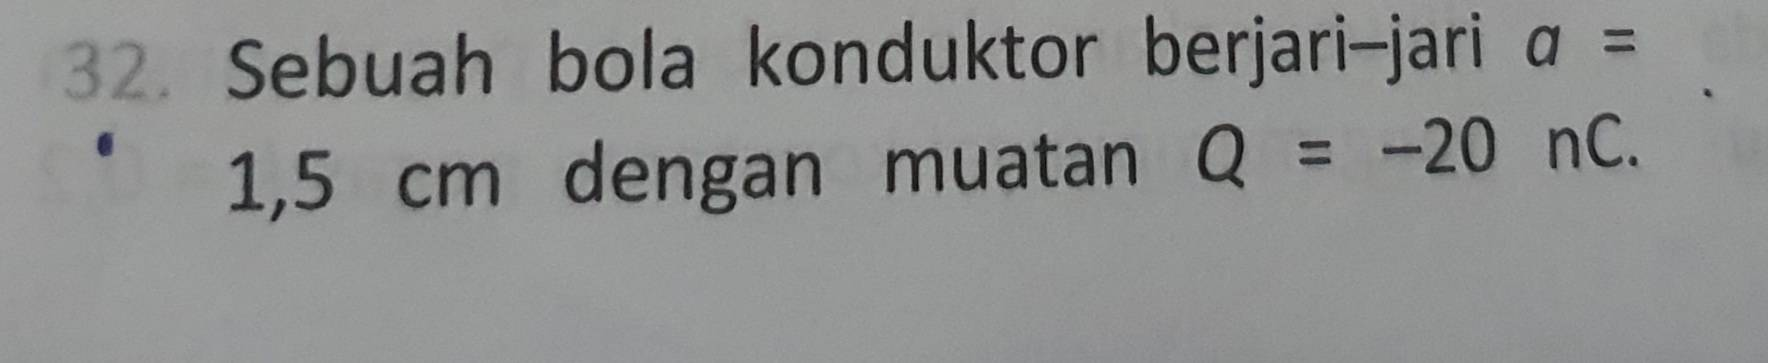
\includegraphics[width=225px]{3.jpg}
    \end{center}

    \begin{center}
        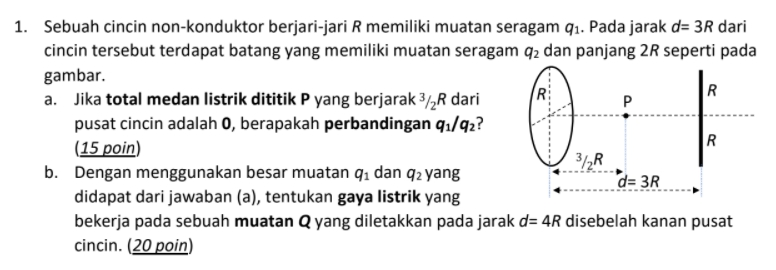
\includegraphics[width=225px]{4.jpg}
    \end{center}

    \begin{center}
        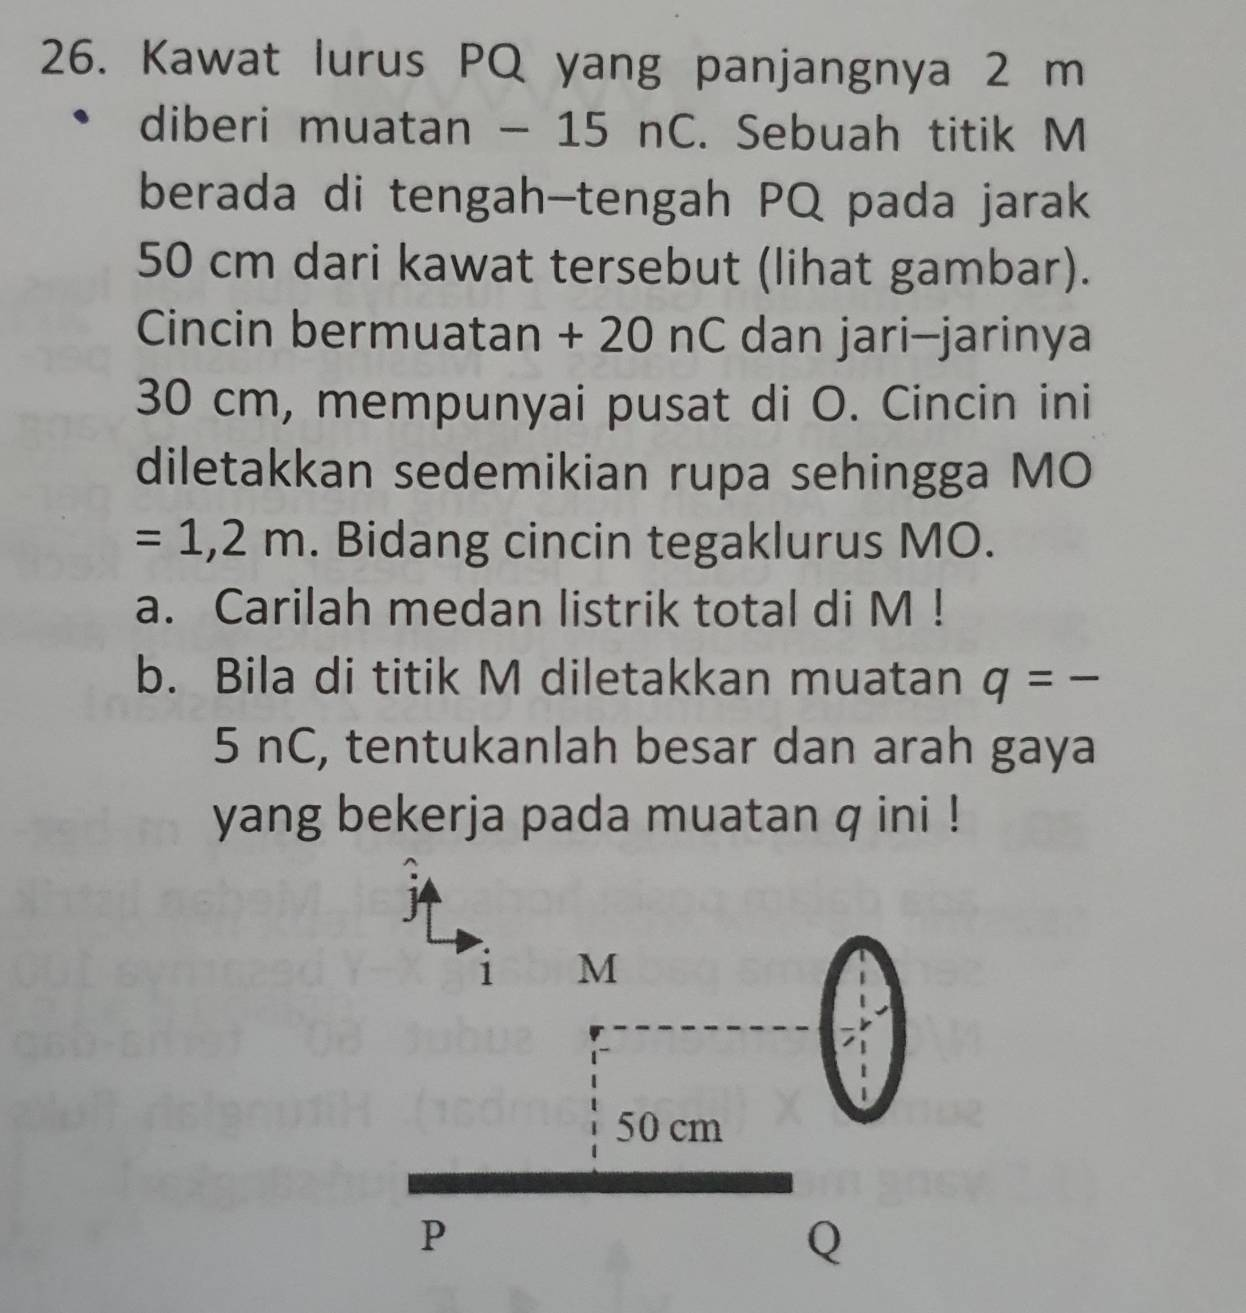
\includegraphics[width=225px]{5.jpg}
    \end{center}

\end{document}
